% Chapter Template

\chapter{Problem Solution} % Main chapter title

\label{Chapter6} % Change X to a consecutive number; for referencing this chapter elsewhere, use \ref{ChapterX}

\lhead{Chapter 6. \emph{Problem Solution}} % Change X to a consecutive
% number; this is for the header on each page - perhaps a shortened title

%----------------------------------------------------------------------------------------
%	SECTION 1
%----------------------------------------------------------------------------------------

\section{Introduction}

%----------------------------------------------------------------------------------------
%	SECTION 2
%----------------------------------------------------------------------------------------
\section{DPF Model Transformation Editor}

\section{Henshin}

\begin{figure}[H]
	\centering
	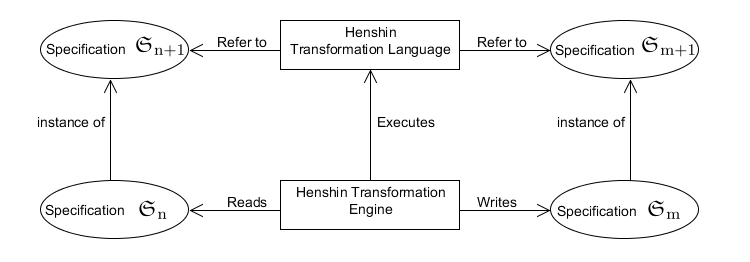
\includegraphics[scale=0.7]{./Figures/TransformationSolutionBasic.png}
	\caption[A specification and some predefined diagrammatic predicate attached]
	{A specification $\spec{S}$\textsubscript{2} with some attached predicates.}
	\label{fig:Simple_Solution}
\end{figure}

\begin{figure}[H]
	\centering
	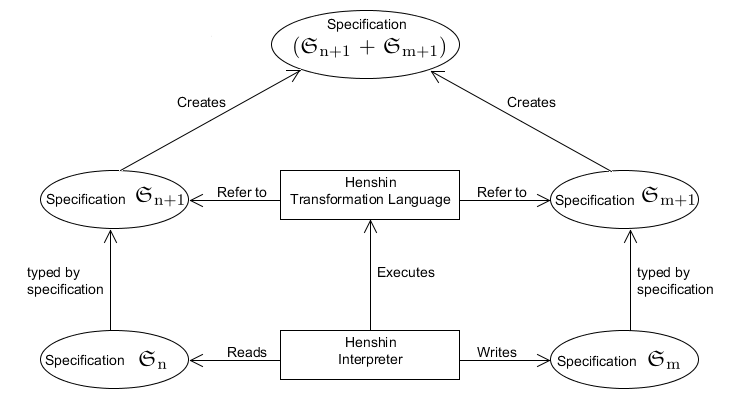
\includegraphics[scale=0.7]{./Figures/TransformationSolution_Correspond.png}
	\caption[Specification for the correspondence objects]
	{The solution expanded with a specification for the correspondence objects.}
	\label{fig:Solution:CorrespondanceObjects}
\end{figure}



\section{Henshin Metamodel}

\section{Integrateing Henshin with DPF Model Transformation Editor}

\section{Henhsin Editor}



